\def\fastrcnn{
    \subsubsection{Mô hình Fast R-CNN}
    Fast R-CNN \cite{girshick2015fast}, được phát triển bởi một trong nhóm tác giả của mô hình R-CNN, và là một phiên bản nâng cấp hơn so với R-CNN giúp phần nào giải quyết được một phần điểm yếu về tốc độ của mô hình R-CNN.

    \noindent
    \textbf{\textit{Kiến trúc mô hình Fast R-CNN}} \\
    Là một phiên bản nâng cấp của mô hình R-CNN, nên Fast R-CNN cũng bao gồm hai thành phần: \\
    - Phần region proposals module \index{region proposals module} mà mô hình Fast R-CNN sử dụng vẫn là thuật toán Selective Search tương tự như R-CNN. \\
    - Phần feature extraction module \index{feature extraction module} của mô hình R-CNN là một mô hình phân lớp ảnh, cụ thể theo \cite{girshick2015fast} là VGG16. \\
    Các thành phần của mô hình Fast R-CNN không có thay đổi gì quá nổi bật so với R-CNN, tuy nhiên, điểm khác biệt mang lại giá trị của Fast R-CNN nằm ở cách mà mô hình này kết hợp hai thành phần trên.

    \begin{figure}[H]
        \centering
        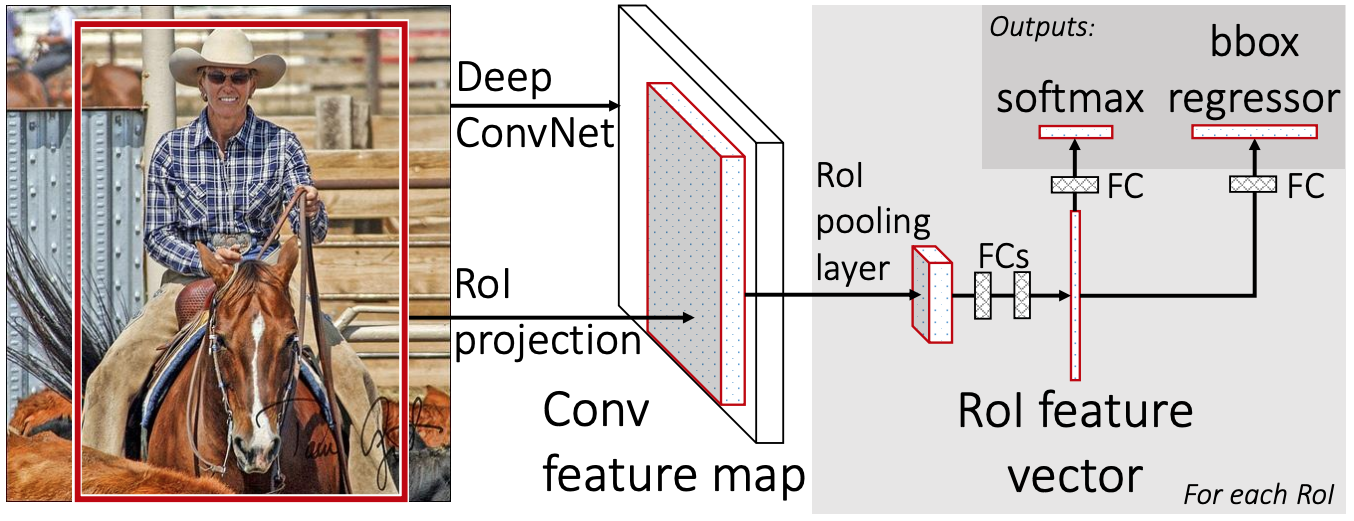
\includegraphics[width=13cm] {images/fast_rcnn_model}
        \caption{Kiến trúc mô hình Fast R-CNN (Nguồn: \cite{girshick2015fast})}
        \label{fig:fast_rcnn_model}
    \end{figure}

    \noindent
    Khác với R-CNN, mô hình Fast R-CNN đưa toàn bộ ảnh ban đầu qua các lớp conv và pooling của feature extraction module \index{feature extraction module} để tạo ra được đặc trưng của toàn bộ ảnh.
    Tiếp theo, với mỗi khu vực mà thuật toán Selective Search đề xuất (các khu vực này, theo \cite{girshick2015fast}, gọi là các \textit{regions of interest} hay \textit{RoIs}), mô hình Fast R-CNN trích xuất từ đặc trưng của toàn bộ ảnh ra đặc trưng đại diện cho khu vực đề xuất đó.
    Cuối cùng, mỗi đặc trưng đại diện cho mỗi khu vực đề xuất được đưa qua các lớp fully-connected và trả hai đầu ra gồm giá trị xác suất khu vực đó là đối tượng nào và giá trị độ lệch của bounding box \index{bounding box}. \\
    Tuy nhiên, có một vấn xảy ra với cách thiết kế mô hình trên, đó là mỗi khu vực đề xuất từ thuật toán Selective Search có kích thước khác nhau, do đó, kích thước của đặc trưng đại diện cho mỗi khu vực đề xuất cũng khác nhau và ta cần các đặc trưng này có cùng kích thước để có thể đưa vào cùng chung các lớp fully-connected.
    Tác giả giải quyết vấn đề này bằng cách xây dựng một lớp mới trong kiến trúc mô hình Fast R-CNN, tên là \textit{RoI pooling}.

    \noindent
    \textbf{\textit{Lớp RoI pooling}} \\
    Trước khi đi sâu vào chi tiết của lớp RoI pooling, ta sẽ cùng bàn luận về lớp pooling thông thường.
    Có hai phương pháp pooling phổ biến là max pooling và average pooling.

    \begin{figure}[H]
        \centering
        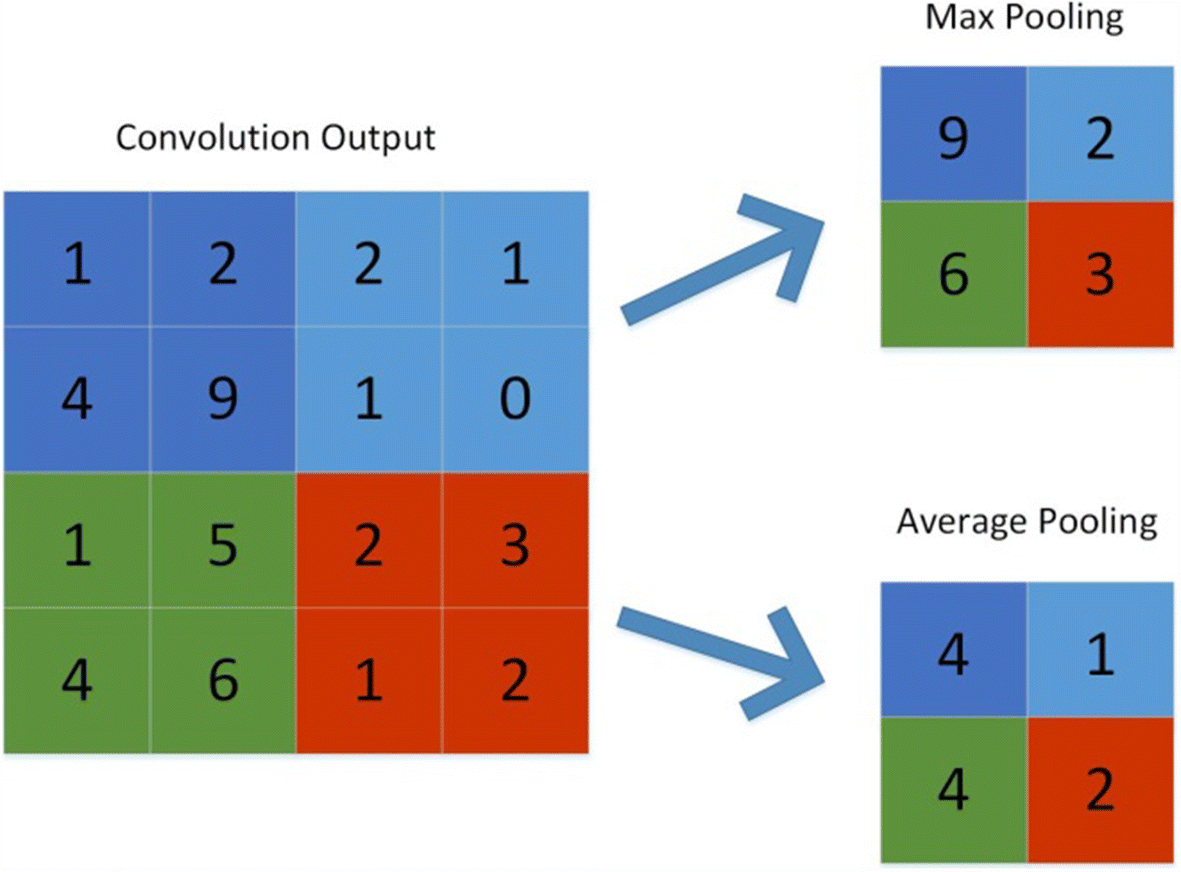
\includegraphics[width=8cm] {images/pooling}
        \caption{Kết quả sau khi thực hiện max pooling và average pooling (Nguồn: media.springernature.com)}
        \label{fig:pooling}
    \end{figure}

    \noindent
    Tuy nhiên, hai phương pháp trên đều có cách thực hiện dựa trên kernel và stride, nghĩa là kích thước của đặc trưng sau khi đi qua lớp pooling phụ thuộc vào kích thước đặc trưng trước khi đi qua lớp pooling, kích thước của kernel pooling và kích thước của stride pooling. \\
    Cụ thể hơn, với một đặc trưng từ lớp conv có kích thước chiều rộng và chiều cao lần lượt là ${W}_{1}$ và ${H}_{1}$ và lớp pooling có kích thước kernel là K, kích thước stride là S, ta sẽ thu được đặc trưng sau khi đi qua lớp pooling này có kích thước chiều rộng và chiều cao lần lượt là ${W}_{2} = \frac{{W}_{1} - (K - 1) - 1}{S} + 1$ và ${H}_{2} = \frac{{H}_{1} - (K - 1) - 1}{S} + 1$.

    \begin{figure}[H]
        \centering
        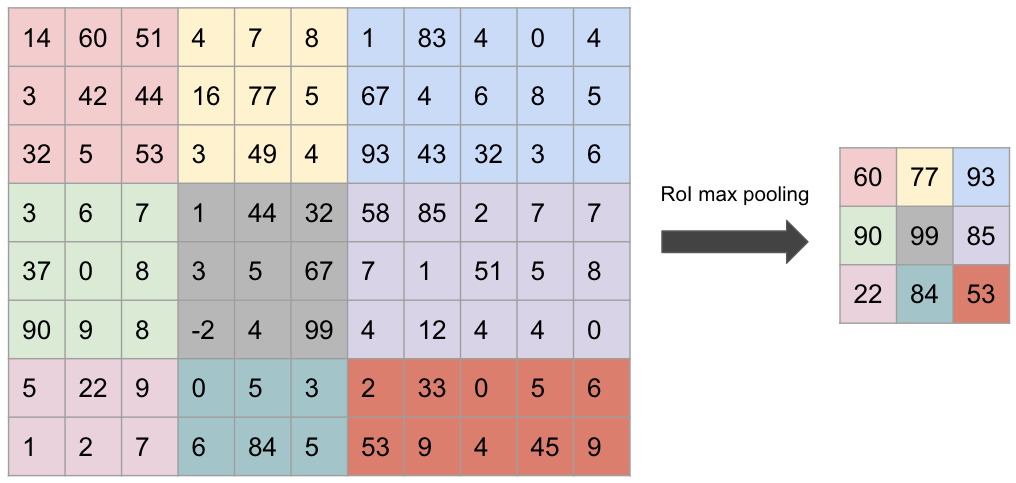
\includegraphics[width=10cm] {images/roi_pooling}
        \caption{Kết quả sau khi thực hiện RoI max pooling}
        \label{fig:roi_pooling}
    \end{figure}

    \noindent
    Trong khi đó, RoIs pooling được giới thiệu bởi tác giả không hoạt động như vậy.
    Thay vì yêu cầu ta phải định nghĩa kích thước kernel và kích thước stride, RoI pooling yêu cầu ta phải định nghĩa kích thước của đặc trưng đầu ra, từ đó, RoI pooling sẽ tính toán và chia đặc trưng đầu vào thành các vùng trước khi thực hiện phép max pooling. \\
    Cụ thể hơn, với một đặc trưng từ lớp conv có kích thước chiều rộng và chiều cao lần lượt là ${W}_{1}$ và ${H}_{1}$ và ta định nghĩa kích thước của đặc trưng đầu ra có kích thước chiều rộng và chiều cao lần lượt là ${W}_{2}$ và ${H}_{2}$, RoI pooling sẽ tính toán được kích thước và vị trí của từng khu vực pooling: \\
    - Theo chiều W, ta có ${W}_{2}$ phần pooling và mỗi phần có kích thước là ${K}_{w} = \lfloor\frac{{W}_{1}}{{W}_{2}}\rfloor$, ngoại trừ phần cuối có kích thước ${K}_{w} + ({W}_{1} - {W}_{2} * {K}_{w})$. \\
    - Theo chiều H, ta có ${H}_{2}$ phần pooling và mỗi phần có kích thước là ${K}_{h} = \lfloor\frac{{H}_{1}}{{H}_{2}}\rfloor$, ngoại trừ phần cuối có kích thước ${K}_{h} + ({H}_{1} - {H}_{2} * {K}_{h})$. \\

    \noindent
    \textbf{\textit{Hàm loss multi-task và cách finetune mô hình Fast R-CNN}} \\
    Một điểm cải tiến khác của mô hình Fast R-CNN so với mô hình R-CNN đó là việc sử dụng hàm loss multi-task và finetune toàn bộ mô hình. \\
    Trong quá trình train mô hình, tác giả lấy ngẫu nhiên N ảnh và lấy ngẫu nhiên $\frac{R}{N}$ RoIs trên mỗi ảnh.
    Nhằm đảm bảo vấn đề về bộ nhớ không xảy ra trong suốt quá trình train, tác giả lựa chọn N = 2 và R = 128.
    Ngoài ra, tác giả cũng đề cập đến một lo ngại khác, đó là việc sử dụng nhiều RoIs trên một số ít ảnh có thể dẫn đến quá trình tối ưu chậm và mất nhiều thời gian để mô hình đạt được điểm hội tụ.
    Tuy nhiên, trong thực tế, điều này đã không xảy ra. \\
    Mô hình Fast R-CNN có hai lớp đầu ra: \\
    - Một là giá trị xác suất một khu vực nào đó là đối tượng nào $p = (p_0, \dots, p_K)$, tương ứng với $K + 1$ lớp đối tượng \index{lớp đối tượng} ($K$ lớp đối tượng \index{lớp đối tượng} từ bộ dữ liệu và 1 lớp background \index{background}). \\
    - Còn lại là giá trị độ lệch bounding box \index{bounding box} của khu vực đó $t^{k} = (t^{k}_{x}, t^{k}_{y}, t^{k}_{w}, t^{k}_{h})$, tương ứng với $K$ lớp đối tượng \index{lớp đối tượng} từ bộ dữ liệu. \\
    Với groundtruth \index{groundtruth} lớp đối tượng \index{lớp đối tượng} $u$ và groundtruth \index{groundtruth} toạ độ bounding box \index{bounding box} $v$, ta có hàm loss multi-task với mỗi RoI như sau:

    \begin{equation}
        \label{eq:fast_rcnn_loss}
        L(p, u, t^u, v) = L_{cls}(p, u) + \lambda [u \ge 1] L_{loc}(t^u, v)
    \end{equation}

    \noindent
    Hàm loss trên gồm các thành phần: \\
    -  $L_{cls}(p, u) = -\log p_u$ là hàm log loss với groundtruth \index{groundtruth} lớp đối tượng \index{lớp đối tượng} $u$ \\
    -  $[u \ge 1]$ là hàm chỉ định. Thành phần này bằng 1 nếu $u \ge 1$ và bằng 0 trong các trường hợp còn lại. Thành phần này tồn tại nhằm loại bỏ phần hàm loss tính toán độ lệch bounding box \index{bounding box} nếu lớp đối tượng \index{lớp đối tượng} $u = 0$ bởi vì khi đó, $u$ đại diện cho lớp background \index{background}. \\
    -  $L_{loc}(t^u, v)$ là hàm loss tính toán độ lệch giữa groundtruth \index{groundtruth} toạ độ bounding box \index{bounding box} $v = (v_{x}, v_{y}, v_{w}, v_{h})$ và bounding box \index{bounding box} dự đoán $t^u = (t^u_{x}, t^u_{y}, t^u_{w}, t^u_{h})$ tương ứng với groundtruth \index{groundtruth} lớp đối tượng \index{lớp đối tượng} $u$. Mỗi bounding box \index{bounding box} được biểu diễn bởi bốn giá trị, x - toạ độ x của góc trái trên, y - toạ độ y của góc trái trên, w - chiều rộng của bounding box \index{bounding box} và h - chiều cao của bounding box \index{bounding box}.
    Công thức cụ thể của thành phần $L_{loc}(t^u, v)$ như sau:

    \begin{equation}
        \label{eq:fast_rcnn_bb_loss}
        L_{loc}(t^u, v) = \sum_{i \in \{{x},{y},{w},{h}\}} {smooth}_{L_1}(t^u_i - v_i)
    \end{equation}

    \noindent
    trong đó:

    \begin{equation}
        \label{eq:fast_rcnn_bb_loss_l1}
        {smooth}_{L_1}(x) =
        \begin{cases}
            0.5x^2& {if} |x| < 1 \\
            |x| - 0.5& {otherwise}
        \end{cases}
    \end{equation}

    \noindent
    Tác giả giải thích việc sử dụng hàm ${smooth}_{L_1}(x)$ bởi vì nó ít nhạy cảm hơn với outliers so với hàm ${L_2}$ được sử dụng trong mô hình R-CNN.
    Ngoài ra, tác giả cũng chuẩn hoá các toạ độ $v$ với trung bình bằng 0 và phương sai đơn vị.
    Giá trị $\lambda$ được tác giả sử dụng nhằm cân bằng giữa hai thành phần loss, và trong các thí nghiệm của mô hình Fast R-CNN, tác giả lựa chọn $\lambda = 1$. \\
    TODO: bổ sung backprop cho pooling \\
    TODO: tăng tốc độ tính toán bằng SVD

    \noindent
    \textbf{\textit{Kết quả của mô hình Fast R-CNN}} \\
    Đầu tiên, kết quả của mô hình Fast R-CNN trên bộ dữ liệu VOC 2007 test đáng chú ý.
    Trong hình \ref{fig:fast_rcnn_results_1}, tác giả xét đến ba cấu hình của mô hình Fast R-CNN, các cấu hình này đều có kiến trúc như nhau (đều sử dụng mô hình VGG16 cho thành phần feature extraction module \index{feature extraction module}) nhưng khác nhau về bộ dữ liệu train mà mỗi cấu hình sử dụng: \\
    - Cấu hình sử dụng bộ dữ liệu train là VOC07 trainval: ký hiệu là \textbf{07} \\
    - Cấu hình sử dụng bộ dữ liệu train là VOC07 trainval nhưng loại đi các dữ liệu khó: ký hiệu là \textbf{07 $\setminus$ diff} \\
    - Cấu hình sử dụng bộ dữ liệu train là sự kết hợp giữa VOC07 trainval và VOC12 trainval: ký hiệu là \textbf{07+12} \\
    Trong nhóm các mô hình so sánh, có kết quả của cấu hình tốt nhất của mô hình R-CNN là R-CNN BB.
    Ngoài ra còn có mô hình SPPnet BB. \\
    Kết quả tất cả các cấu hình của Fast R-CNN đều cho kết quả trên mAP tốt hơn khoảng 4\% so với kết quả của R-CNN BB hay SPPnet BB.
    Trong đó, kết quả của cấu hình \textbf{07 + 12} mô hình Fast R-CNN cho kết quả tốt nhất.
    Tuy nhiên, vẫn tồn tại một số lớp đối tượng \index{lớp đối tượng} mà chỉ số AP của cấu hình này làm chưa tốt so với các cấu hình khác hay các mô hình khác như lớp \textit{bike, bottle, plant ...}.

    \begin{figure}[H]
        \centering
        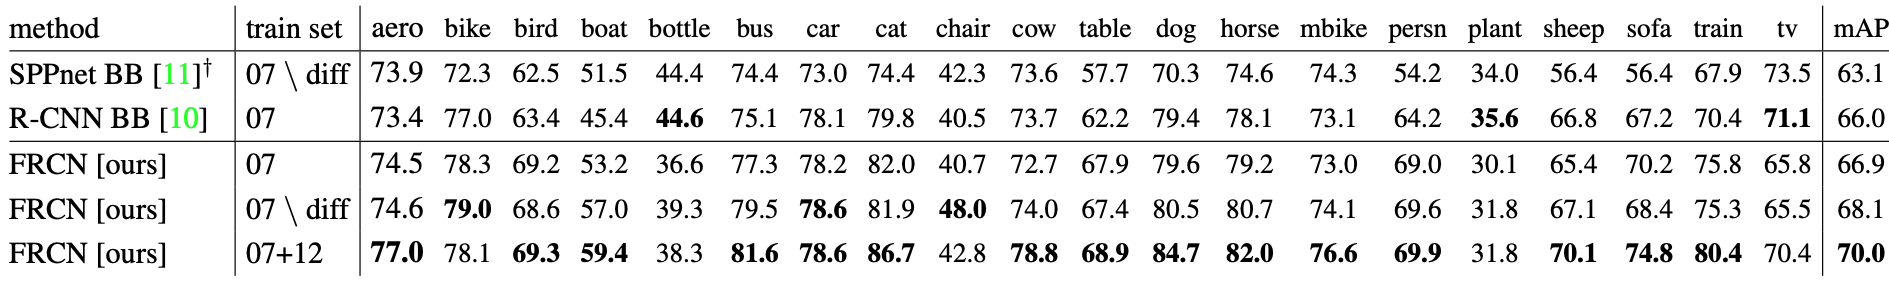
\includegraphics[width=15cm] {images/fast_rcnn_results_1}
        \caption{Kết quả của mô hình Fast R-CNN với các cấu hình khác nhau cùng các mô hình khác trên bộ dữ liệu VOC 2007 test. (Nguồn: \cite{girshick2015fast})}
        \label{fig:fast_rcnn_results_1}
    \end{figure}

    \noindent
    Tiếp theo, mô hình Fast R-CNN cũng có kết quả tốt trên bộ dữ liệu VOC 2010 test.
    Trong hình \ref{fig:fast_rcnn_results_2}, tác giả xét đến hai cấu hình của mô hình Fast R-CNN, các cấu hình này đều có kiến trúc như nhau (đều sử dụng mô hình VGG16 cho thành phần feature extraction module \index{feature extraction module}) nhưng khác nhau về bộ dữ liệu train mà mỗi cấu hình sử dụng: \\
    - Cấu hình sử dụng bộ dữ liệu train là VOC12 trainval: ký hiệu là \textbf{12} \\
    - Cấu hình sử dụng bộ dữ liệu train là sự kết hợp giữa VOC07 trainval, VOC07 test và VOC12 trainval: ký hiệu là \textbf{07 ++ 12} \\
    Trong nhóm các mô hình so sánh, có kết quả của cấu hình tốt nhất của mô hình R-CNN là R-CNN BB.
    Ngoài ra còn có các mô hình BabyLearning (được train với bộ dữ liệu độc quyền) và mô hình SegDeepM (được train với bộ dữ liệu VOC 12 trainval bổ sung thêm các groundtruth \index{groundtruth} segmentation). \\
    Kết quả của cấu hình \textbf{07 ++ 12} mô hình Fast R-CNN cho mAP cao hơn khoảng 2\% so với các cấu hình và mô hình khác.
    Tuy nhiên, vẫn tồn tại một số lớp đối tượng \index{lớp đối tượng} mà chỉ số AP của cấu hình này làm chưa tốt so với các cấu hình khác hay các mô hình khác như lớp \textit{bottle, plant, sheep, tv ...}.

    \begin{figure}[H]
        \centering
        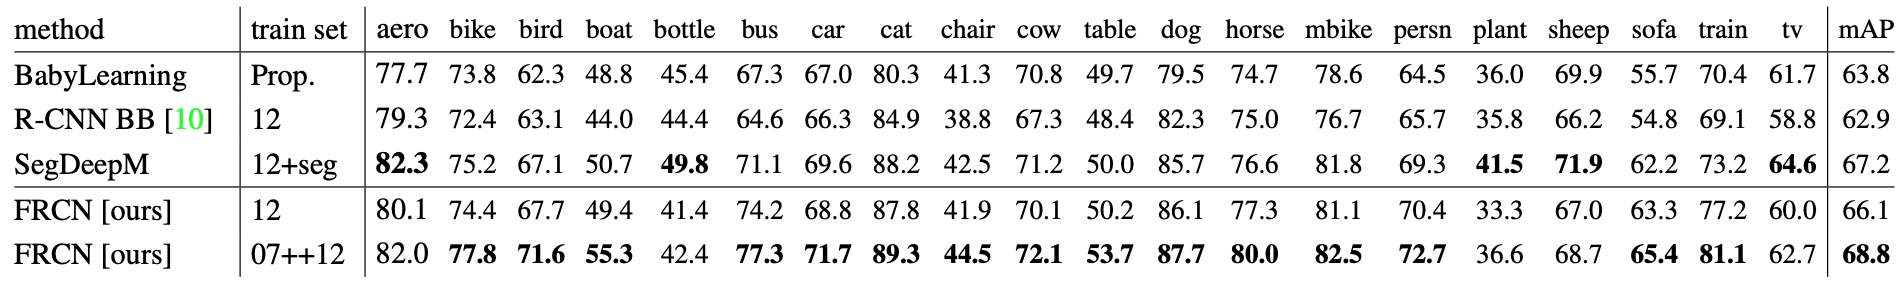
\includegraphics[width=15cm] {images/fast_rcnn_results_2}
        \caption{Kết quả của mô hình Fast R-CNN với các cấu hình khác nhau cùng các mô hình khác trên bộ dữ liệu VOC 2010 test. (Nguồn: \cite{girshick2015fast})}
        \label{fig:fast_rcnn_results_2}
    \end{figure}

    \noindent
    Đối với bộ dữ liệu VOC 2012 test, tác giả vẫn sử dụng hai cấu hình \textbf{12} và \textbf{07 ++ 12} của mô hình Fast R-CNN từ kết quả trên. Nhóm các mô hình so sánh gồm cấu hình R-CNN BB của mô hình R-CNN, mô hình BabyLearning (được train với bộ dữ liệu độc quyền) và mô hình NUS\_NIN\_c2000. \\
    Trong hình \ref{fig:fast_rcnn_results_3}, kết quả của cấu hình \textbf{07 ++ 12} mô hình Fast R-CNN cho mAP cao hơn khoảng 3-5\% so với các cấu hình và mô hình khác. \\
    Kết quả này vẫn tồn tại một số lớp đối tượng \index{lớp đối tượng} mà chỉ số AP của cấu hình này làm chưa tốt so với các cấu hình khác hay các mô hình khác như lớp \textit{bottle, plant}.

    \begin{figure}[H]
        \centering
        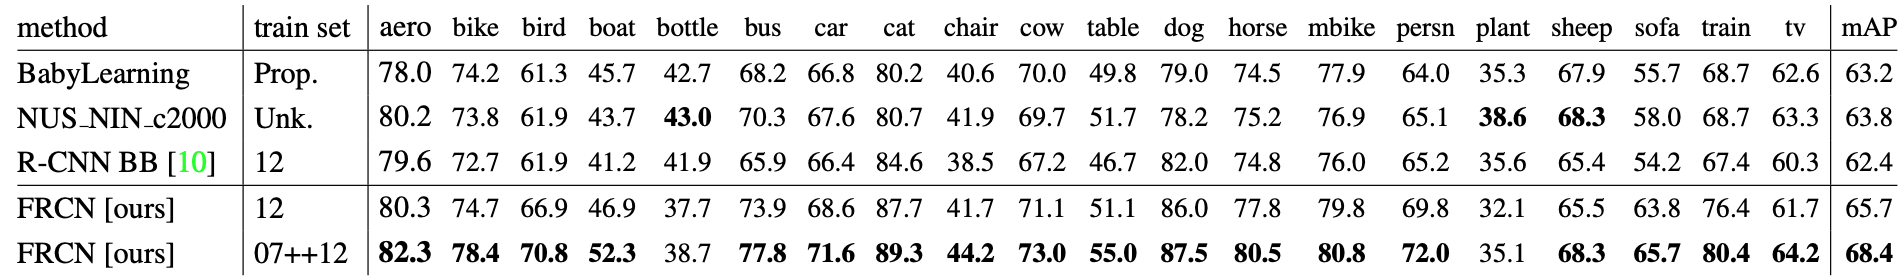
\includegraphics[width=15cm] {images/fast_rcnn_results_3}
        \caption{Kết quả của mô hình Fast R-CNN với các cấu hình khác nhau cùng các mô hình khác trên bộ dữ liệu VOC 2012 test. (Nguồn: \cite{girshick2015fast})}
        \label{fig:fast_rcnn_results_3}
    \end{figure}

    \noindent
    Cuối cùng, tác giả chia sẻ kết quả khi so sánh về mặt tốc độ trong quá trình train và quá trình test và đây là một trong số những thành quả chính. \\
    Trong hình \ref{fig:fast_rcnn_results_4}, tác giả so sánh tốc độ xử lý mỗi ảnh trong quá trình train và test giữa mô hình Fast R-CNN, R-CNN và SPPnet.
    Cụ thể hơn, trong quá trình train, thời gian train của mô hình Fast R-CNN giảm tới 8.8 lần so với mô hình R-CNN.
    Trong quá trình test, thời gian mà mô hình Fast R-CNN xử lý một ảnh nhanh hơn tới 146 (khi không sử dụng SVD) và tới 213 lần (khi sử dụng SVD) so với mô hình R-CNN.
    Không những thế, với việc cải thiện đáng kể tốc độ train và test, kết quả về độ chính xác của Fast R-CNN vẫn tốt hơn so với R-CNN khi so sánh trên chỉ số mAP.

    \begin{figure}[H]
        \centering
        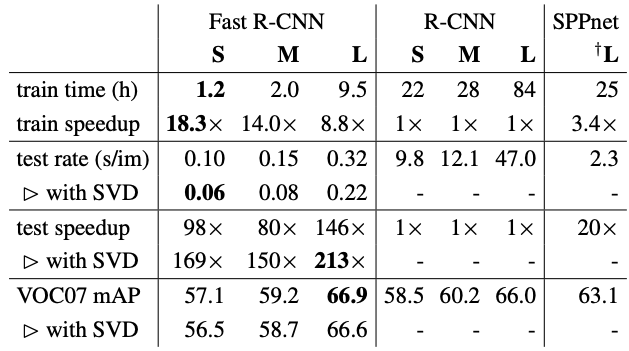
\includegraphics[width=10cm] {images/fast_rcnn_results_4}
        \caption{Kết quả so sánh về mặt tốc độ và độ chính xác giữa các cấu hình khác nhau của mô hình Fast R-CNN, R-CNN và SPPnet. (Nguồn: \cite{girshick2015fast})}
        \label{fig:fast_rcnn_results_4}
    \end{figure}

    \noindent
    \textbf{\textit{Vấn đề tồn đọng của mô hình Fast R-CNN}} \\
    Những kết quả vượt bậc về mặt tốc độ của mô hình Fast R-CNN đã giải quyết được vấn đề tồn đọng của R-CNN trong khi vẫn duy trì được độ chính xác cao.
    Tuy nhiên, kiến trúc của mô hình Fast R-CNN vẫn phụ thuộc vào một thuật toán đề xuất khu vực như Selective Search và điều này tạo động lực để các nhà nghiên cứu xây dựng mô hình học sâu thay thế cho các thuật toán này.
}